\chapter*{Aufgabe 1: Pointer}


\section*{1.a}
Stellen Sie dar, welche Ausgabe das nachfolgend dargestellte Programm erzeugt.\\
\begin{lstlisting}
H
e
l
l
o
Erster Wert von i war 5! Korrekt ?
H
I
J
K
L
Erster Wert von i war 0! Korrekt ?
\end{lstlisting}

\section*{1.b}
Geben Sie weiterhin die Hexadezimaldarstellung der Adressen sowie bei
Zeigern den Inhalt, auf den er zeigt, an. Erweitern Sie hierfür das Programm durch
printf-Anweisungen oder verwenden Sie den Debugger.	\\

\begin{lstlisting}
Adresse i: 010FFCE4
Wert i: 5

Adresse first_i: 010FFCCC
Wert first_i: 0

Adresse first_i_ptr: 010FFCD8
Wert first_i_ptr: 010FFCE4
Wert von Adresse 010FFCE4: 5

Adresse onechar: 010FFC4B
Wert onechar: M

Adresse strptr: 010FFC54
Wert strptr: 010FFC65
Wert von Adresse 010FFC65:  World!
\end{lstlisting}
\newpage
\thispagestyle{fancy}
\section*{2.a}
Zeichnen Sie graphisch die Zeigerabhängigkeiten auf.\\
\begin{center}
	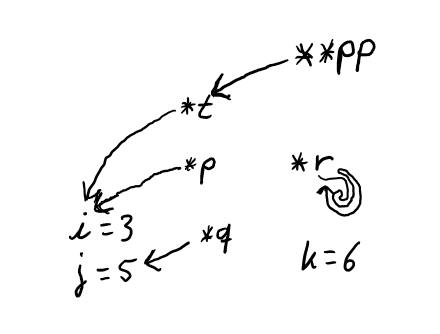
\includegraphics[width=300pt]{img/pointer.png}
\end{center}
\section*{2.b}
\begin{lstlisting}
wert = (p == i);
\end{lstlisting}
Wert ist = 0. Da bei p nicht der Wert, sondern die Adresse betrachtet wird sind nicht beide echt gleich.
\begin{lstlisting}
wert = *p / *q;
\end{lstlisting}
Hier wird 3/5 gerechnet und nur in ganzen Zahlen dargestellt, was hier 0 ist. Falls kein Leerzeichen zwischen / und *p steht denkt das Programm, es wird auskommentiert
\begin{lstlisting}
wert = *p / *q + 3;
\end{lstlisting}
Hier wird zu dem Ergebnis 3 von eben eine 3 hinzuaddiert, deshalb ist das Resultat 3.
\begin{lstlisting}
wert = **&p;
\end{lstlisting}
Wert ist = 3. Da der Wert hinter der Adresse auf die **p zeigt dargestellt wird.
\begin{lstlisting}
wert = *(r = &k);
\end{lstlisting}
Wert ist = 6. r wird auf die Adresse von k gesetzt und dann als Pointer zeigt r auf die Adresse von k mit dem Wert 6.
\begin{lstlisting}
wert = *(r = &k) = *p**q;
\end{lstlisting}
Wert ist = 15. Zuerst wird *r auf die Adresse von k gerichtet, dann wird die Adresse von k auf den Wert 15 (von 3(p)*5(q)) gesetzt und am Ende wir „wert“ diesem Wert gleichgesetzt.
\begin{lstlisting}
wert = *p***pp;
\end{lstlisting}
Wert ist = 9. Der Wert auf den p zeigt, wird mit dem Wert auf den q zeigt multipliziert und auf „wert“ gespeichert.


